\newgeometry{left=4.5cm, right=4.5cm,bottom=4cm, top=4cm}
\chapter{The ATLAS Detector at the LHC}\label{chap:detector}
 \vspace{0.5cm}

The Large Hadron Collider (LHC) located at the European Organization for Nuclear Research (CERN)
is  the largest particle collider facility in the world. The ATLAS experiment is one of the several experiment situated 
at the LHC, it is a general-purpose detector dedicated to explore a wide range of physiscs topics, from
precision measurements of known Standard Model processes to the search for physics beyond the Standard Model. 
Proton-proton collision data recorded by the ATLAS experiment  has been used in this thesis 
for the search for the neutral MSSM Higgs bosons.

This chapter is organized as follows: the design and performance of the LHC  are summarized in 
Section~\ref{sec:lhc} (based on Ref.~\cite{LHC}),  while a description of the  ATLAS detector  is given 
in Section~\ref{sec:atlas} (based on Ref.~\cite{ATLASDetector}).


\restoregeometry
\clearpage



\section{The Large Hadron Collider}\label{sec:lhc}
The LHC is a superconducting hadron syncrotron  collider. It is  installed in the tunnel of the former LEP electron-positron collider
and has $\sim 27$ km circumference.
LHC is designed to collide proton beams with a centre-of-mass energy of 14 TeV and an unprecedented luminosity of 
$10^{34} ~ cm^{-2} s^{-1}$. It can also collide heavy ions (lead) with an energy of 2.8 TeV per nucleon and 
a peak luminosity of $10^{27} ~ cm^{-2} s^{-1}$. 

The LHC provides proton-proton collision for several experiments, the most relevant for the physics program  are the ATLAS, CMS~\cite{cms},
LHCb~\cite{lhcb} and ALICE~\cite{alice} experiments. 
Figure~\ref{fig:LHC} shows the layout of the CERN accelerator complex, the  protons follows several acceleration steps before injection in the LHC machine.
First a linac accelerator ($Linac\,2$) accelerates the protons to an energy of 50~MeV, then they are injected in the \emph{booster} which accelerates them
further to 1.4~GeV. The energy is increased to 25~GeV and successively to 450~GeV by means of two syncrotron accelerators, the \emph{Proton Syncrotron} (PS)
and the \emph{Super Proton Synctrotron} (SPS). Finally, two proton beams are  injected with opposite direction into the LHC 
where they reach their final erergy.

The LHC beams are costituited by bunches of protons which are housed in two separate vacuum pipes. 
Radiofrequency cavities are employed  to accelerate the protons,
while superconductig magnets bends and focuses the bunches.
The LHC is designed to accelerate up to 2835 bunches per beam, each of them containing $\sim 10^{11}$ protons.
The nominal bunch spacing allows collision every 25~ns representing a real challenge for any read-out electronics.

In 2010, fist collisions took place at the LHC between proton beams of energy of 3.5~TeV. The LHC was succesfully in 
operation during years 2011 and 2012, beam of protons were initially delivered with energies of 3.5~TeV  which was increased to 4~TeV in 2012.
Peak luminosities of about $4\times10^{33} ~ cm^{-2}s^{-2}$ and $8\times10^{33} ~ cm^{-2}s^{-2}$  have been reached 
during years 2011 and 2012 respectively. The ATLAS experiment recorded in fully operational conditions an integrated luminosity of 4.57~$fb^{-1}$ 
during year 2011, while an integrated luminosity of 20.3~$fb^{-1}$ was recorded during year 2012.
Data recordered during  these two years  led to one of the major mailstone in particle physics, the discovery in 2012 of a Higgs boson.





\begin{figure}[tp]
     \begin{center}

            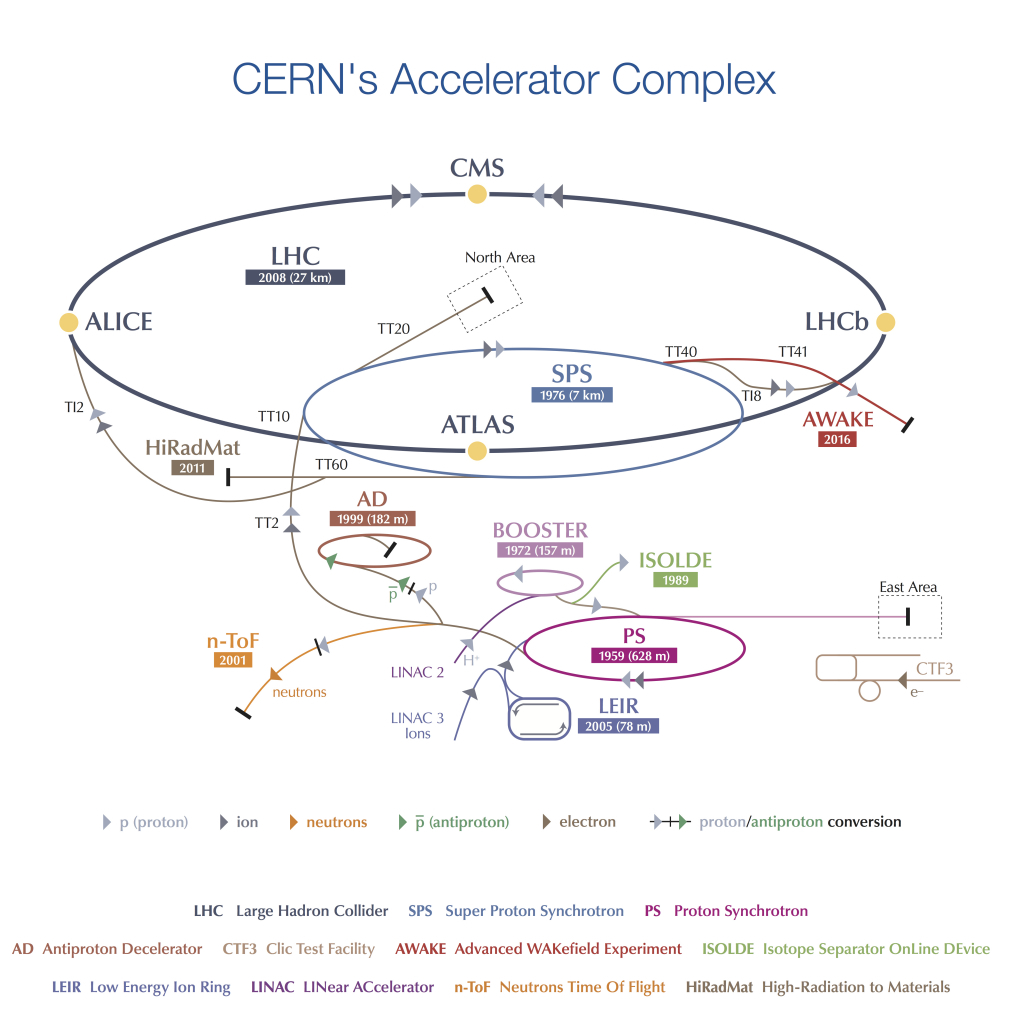
\includegraphics[width=\textwidth]{figure/LHC2.jpg}

    \end{center}
    \caption{Illustration of the CERN accelerator complex~\cite{lhcImage}. The acceleration of protons starts with Linac2 followed by the
	acceleration in the Booster. The Proton Syncrotron (PS) and the Super Proton Syncrotron (SPS) accelerate further the protons before
	final injection into the LHC  machine.}


   \label{fig:LHC}
\end{figure}


\section{The ATLAS Detector}\label{sec:atlas}
The ATLAS detector is a multi-purpose detector which aim to explore a wide range of physiscs topics. The physics programme of the ATLAS experiment ranges from 
precision measurements of known Standard Model processes to the search for physics beyond the Standard Model in a large variety of scenarios.
The ATLAS detector is designed to satisfy the tight requirements on particle identification and acuracy imposed by the physics goals.
A schematic view of the ATLAS detector is shown in Figure~\ref{fig:atlas}. ATLAS is $44\,m$ long and $25\,m$ high, it has a typical design for a collider 
experiments with a forward-backward symmetry with respect the interaction point. It consist of four sub-detector which are built cylindrically around the
beam pipe, going from the inside to outside they are: an Inner Detector tracker, an electromagnetic calorimeter, an hadronic calorimeter and finally
a muon spectrometer sourrounds the whole experiment. Each of these sub-detector is briefly described in what follows based on  Ref.~\cite{ATLASDetector}.


\begin{figure}[tp]
     \begin{center}

            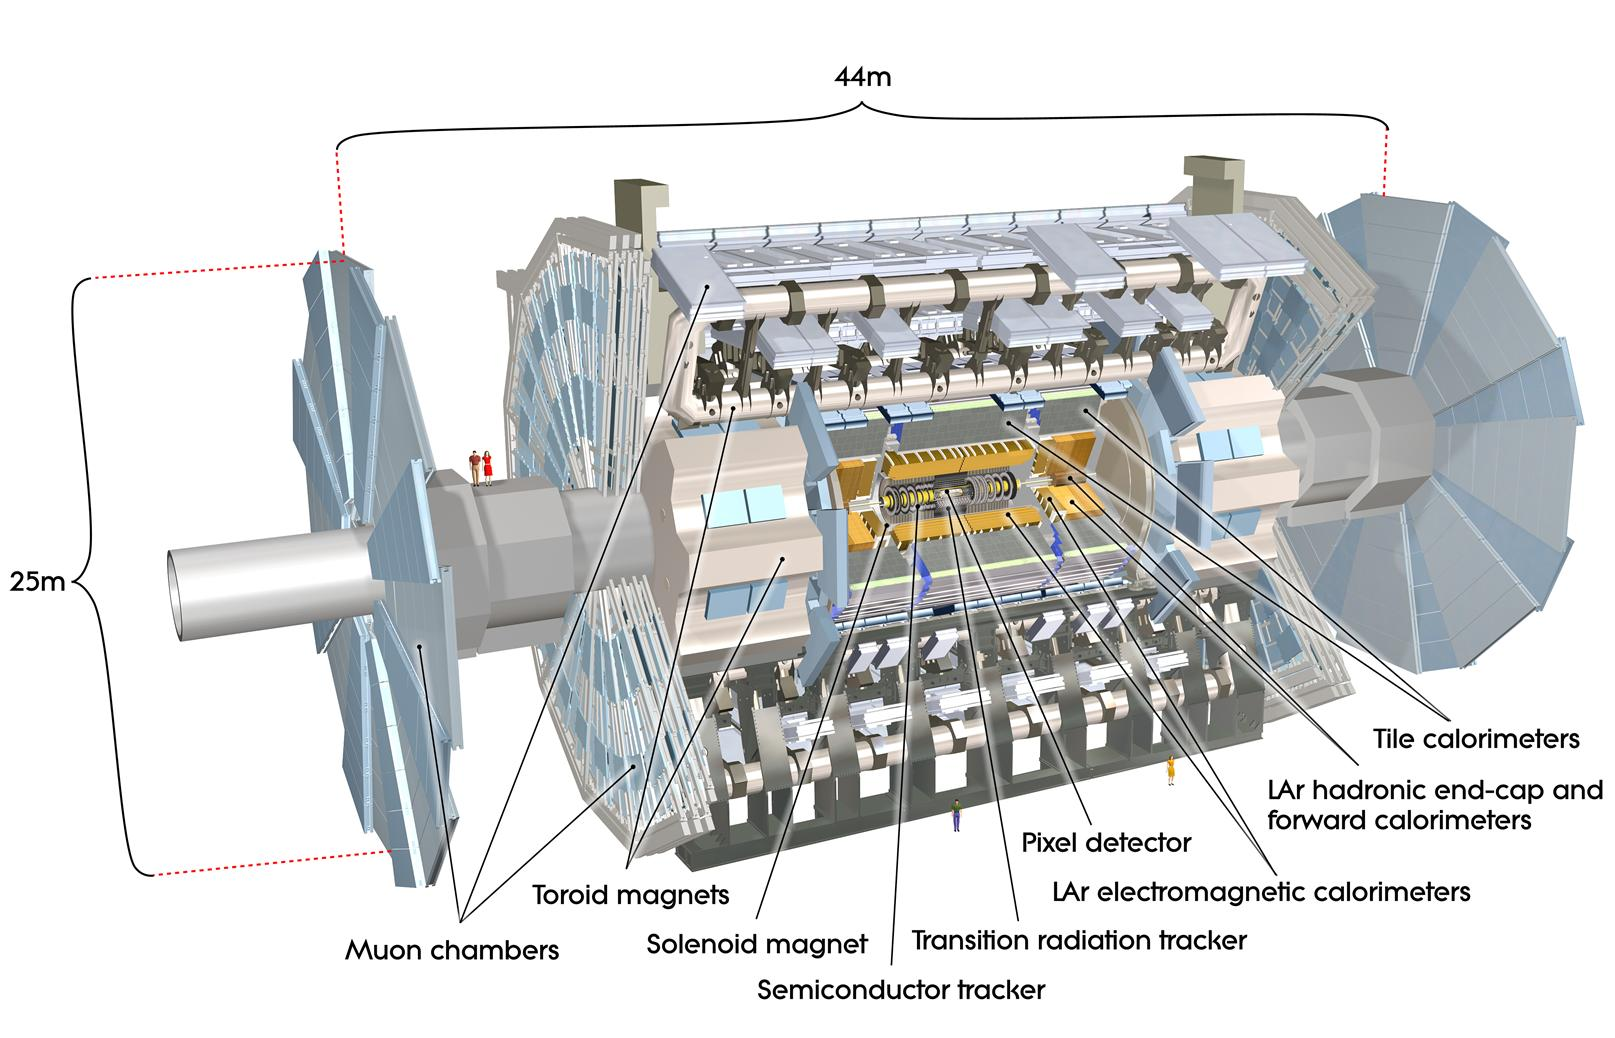
\includegraphics[width=\textwidth]{figure/ATLAS.jpeg}

    \end{center}
    \caption{Cut-away view of the ATLAS detector with its sub-detectors system.  Ref.~\cite{ATLASDetector}.}



   \label{fig:atlas}
\end{figure}


\subsection{The ATLAS coordinate system}
The ATLAS coordinate system has its origin in the interaction region. The $z-$axis is pointing along the beam direction,
the $y-$axis is pointing upwards and the $x-$axis towards the center of the LHC ring. The angle $\phi$ is defined in the plane orthogonal
to the beam axis, starting from the positve side of the $x-$axis. The angle $\theta$ is instead defined with respect to the $z-$axis.
A commonly used spatial coordinate in  experiments at collider is the rapidity $y$:
\begin{equation}
y ~ = ~ 1/2 \cdot \ln \left( \frac{E + p_{z}}{E - P_z} \right) 
\end{equation}
The difference in the rapidity of two particles is independent of Lorentz boosts along the beam axis. In the limit of $\beta$ approaching to one 
or for massless particle the rapidity tend to the pseudorapidity $\eta$:
\begin{equation}
\eta ~ = ~ 1/2 \cdot \ln \left( \frac{\theta}{2} \right) 
\end{equation}
Given the symmetry of the ATLAS detector with respect to the interaction point, the detector is divided in two regions called \emph{barrel} 
for $|\eta| \apprle 1.5$ (depending on the considered detector) 
and \emph{endcap} for larger~$\eta$. In ATLAS the angular separation between two particle is commonly measured by 
$\Delta R ~=~\sqrt{\Delta \eta^2 + \Delta \phi^2}$. 
%Given the symmetry 
%of the ATLAS detector, it is divided in two regions, barrel and endcap.

\subsection{The Inner Detector}

\begin{figure}[tp]
     \begin{center}

            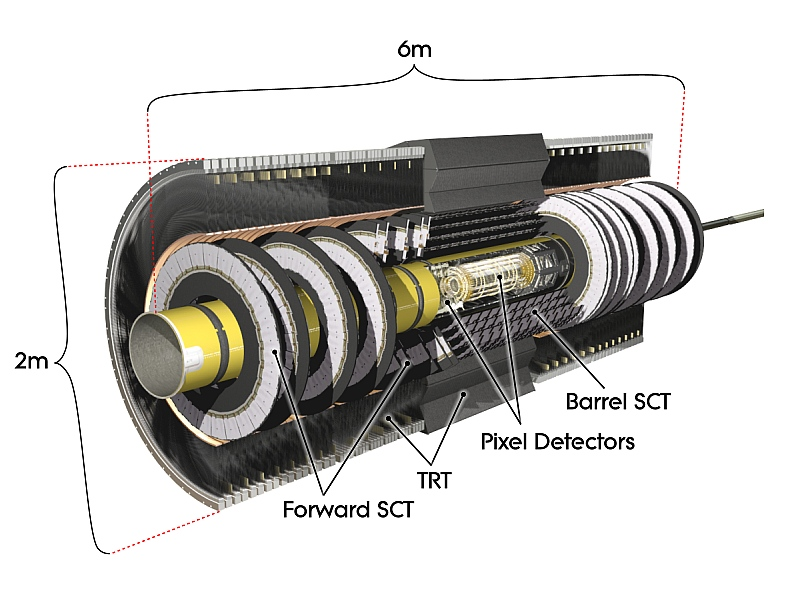
\includegraphics[width=0.7\textwidth]{figure/Inner_detector.jpg}

    \end{center}
    \caption{Cut-away view of the ATLAS Inner Detector tracker. Ref.~\cite{ATLASDetector}.}

   \label{fig:atlasID}
\end{figure}


The Inner Detector (ID) performs track reconstruction  and momentum measurements of charged particles, it has a total lenght of $5.3\,m$ and a diameter of $2.5\,m$.
The momentum measurment is performed by measuring the tracks curvature in a $2\,T$ magnetic field generated by 
a super-conducting solenoid. The layout of the Inner Detector is illustrated in Figure~\ref{fig:atlasID},
it consist of three independent detector modules with fine granularity
covering the region $|\eta| < 2.5$. The innermost of these detectors is the Pixel detector,
which consist of three cylindrical layers of pixel silicon sensors in the barrel and three disks in the endcap region. The closest layer of pixels to the beam pipe is
referred to as the B-layer. The spatial resolution of the pixel sensors is $10\,\mu m$ in the transverse and $115\,\mu m$ in the longitudinal
direction with respect to the beam pipe.

The Semi-Conductor Tracker (SCT) surrounds the Pixel detector with four cilindrical layers of silicon microstrip sensor in the barrel
and nine disks in the  endcap region. The spatial resolution achieved by the SCT is of $17\,\mu m$ in the transverse and $590\,\mu m$ in the longitudinal direction 
respectively.

The outermost detector module is the Transition Radiation Tracker (TRT). It is composed of $4\,mm$ diameter Kapton straw tubes
with a tungsten wire in their center. The tube is filled with a gas mixture which allows the detection of transition 
radiation photons. This detector can only measure position along the transverse direction.

% is t used in
%conjunction with the straw tubes of the Transition Radiation Tracker (TRT), offer these features.
%The precision tracking detectors (pixels and SCT) cover the region
%|η| < 2.5. In the barrel region, they are arranged on concentric cylinders around the beam axis
%while in the end-cap regions they are located on disks perpendicular to the beam axis. The highest
%granularity is achieved around the vertex region using silicon pixel detectors. The pixel layers are
%segmented in R − φ and z with typically three pixel layers crossed by each track. All pixel sensors
%are identical and have a minimum pixel size in R − φ × z of 50 × 400 μm2 . The intrinsic accuracies
%in the barrel are 10 μm (R − φ ) and 115 μm (z) and in the disks are 10 μm (R − φ ) and 115 μm (R).
%The pixel detector has approximately 80.4 million readout channels. For the SCT, eight strip layers
%(four space points) are crossed by each track. In the barrel region, this detector uses small-angle
%(40 mrad) stereo strips to measure both coordinates, with one set of strips in each layer parallel to
%the beam direction, measuring R − φ . They consist of two 6.4 cm long daisy-chained sensors with
%a strip pitch of 80 μm. In the end-cap region, the detectors have a set of strips running radially and
%a set of stereo strips at an angle of 40 mrad. The mean pitch of the strips is also approximately
%80 μm. The intrinsic accuracies per module in the barrel are 17 μm (R − φ ) and 580 μm (z) and in
%the disks are 17 μm (R − φ ) and 580 μm (R). The total number of readout channels in the SCT is
%approximately 6.3 million.




\subsection{The Calorimeter System}

\begin{figure}[tp]
     \begin{center}

            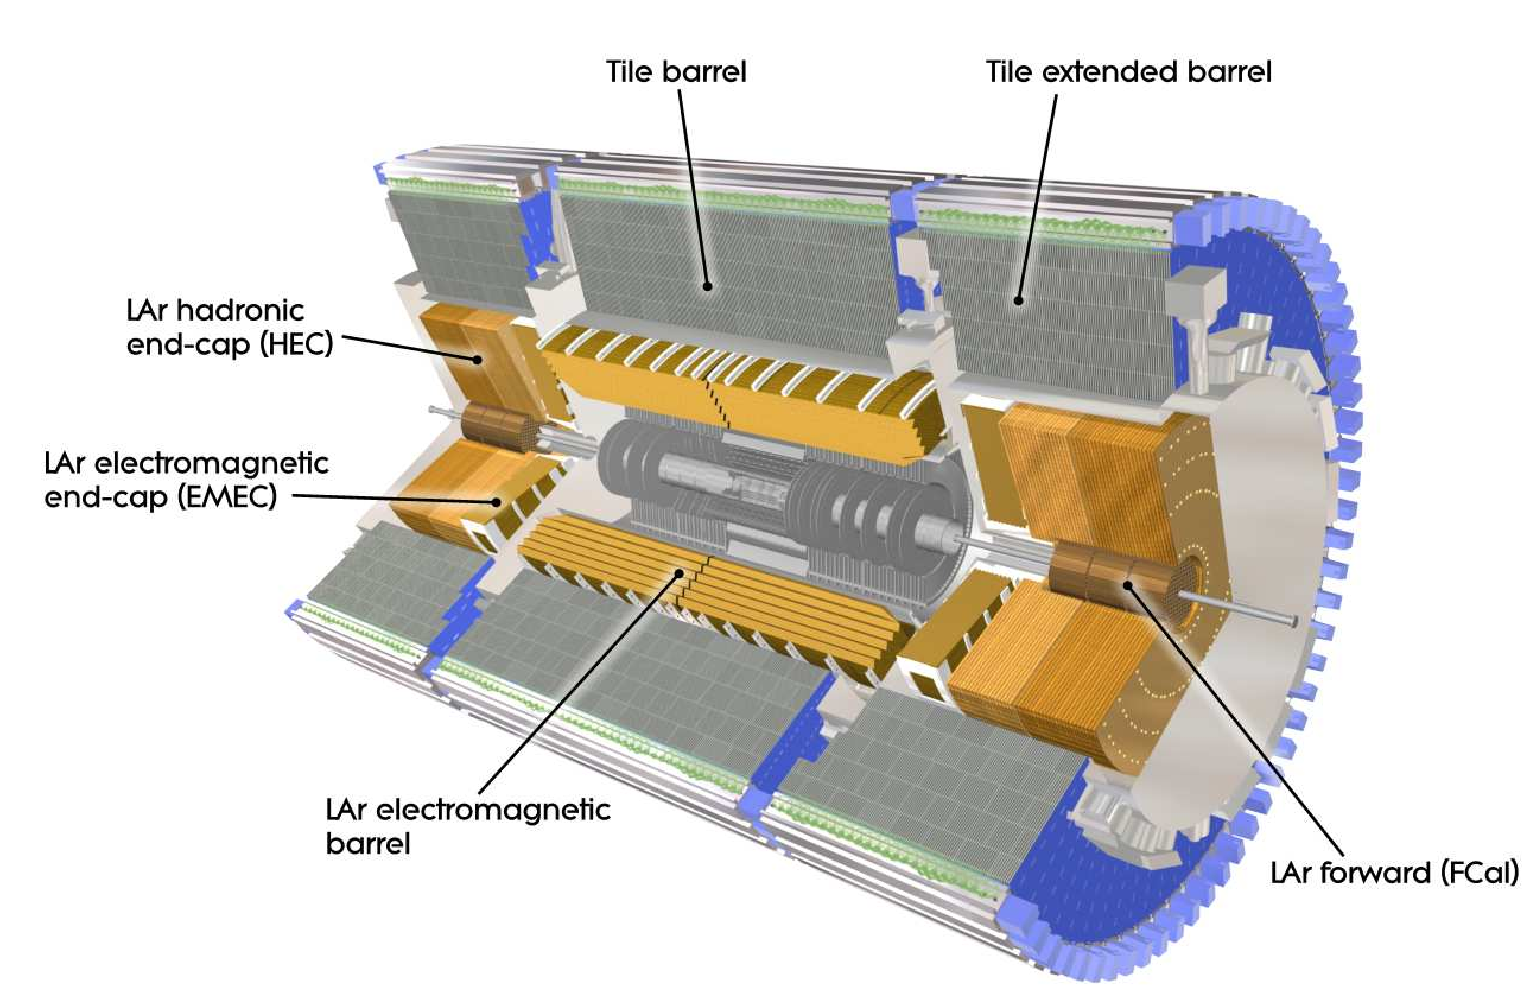
\includegraphics[width=0.7\textwidth]{figure/Calo.png}

    \end{center}
    \caption{Cut-away view of the ATLAS calorimeter system. Ref.~\cite{ATLASDetector}.}



   \label{fig:atlasCal}
\end{figure}

An illustration of the ATLAS calorimeter system is shown in Figure~\ref{fig:atlasCal}, it consist of an electromagnetic calorimeter (EM) sourraunded by an hadronic 
calorimeter.  These calorimeters cover the range $|\eta| < 4.9$ using different techniques suited to the
widely varying  radiation environment over this large $\eta-$range. Both these calorimeters are sampling calorimeters, they are builded alternatig
active material, which performs the detector response and a passive absorber.
The total detector thickness at $\eta = 0$ is 9.7 interaction lenght. 

The EM Lar calorimeter is ideally suited for precision measurements of electrons and photons.  It uses lead as absorber material and liquid argon 
as active material. It extends up to $|\eta| < 3.2$.

The hadronic calorimeter has a coarser granularity with respect the EM calorimeter and it is suited  for
jet reconstruction and $\met$ measurements. The hadronic calorimeter is divided in three sub-detectors which make use of different technology to cope 
with the changing radiation environment as a function of $\eta$. The Tile calorimeter covers region in pseudorapidity up to $|\eta| < 1.7$, it uses 
scintillating tiles as active material and steel as absorber. 
In the forward region ATLAS is instrumented with a Lar hadronic endcap calorimeter (HEC),
which extends up to $|\eta| < 3.2$ and uses argon as active material and copper as absorber. The region in $3.1 <|\eta| < 4.9$ is istrumented instead with a 
liquid argon Forward CALorimeter (FCAL), 
%this provides clear benefits in terms of uniformity of the calorimetric coverage as well as
%reduced radiation background levels in the muon spectrometer. 
which is divided in three modules, the closest to the interaction point uses 
copper as absormer material, while the other two uses tungsten.



\subsection{The Muon Spectrometer}
\begin{figure}[tp]
     \begin{center}

            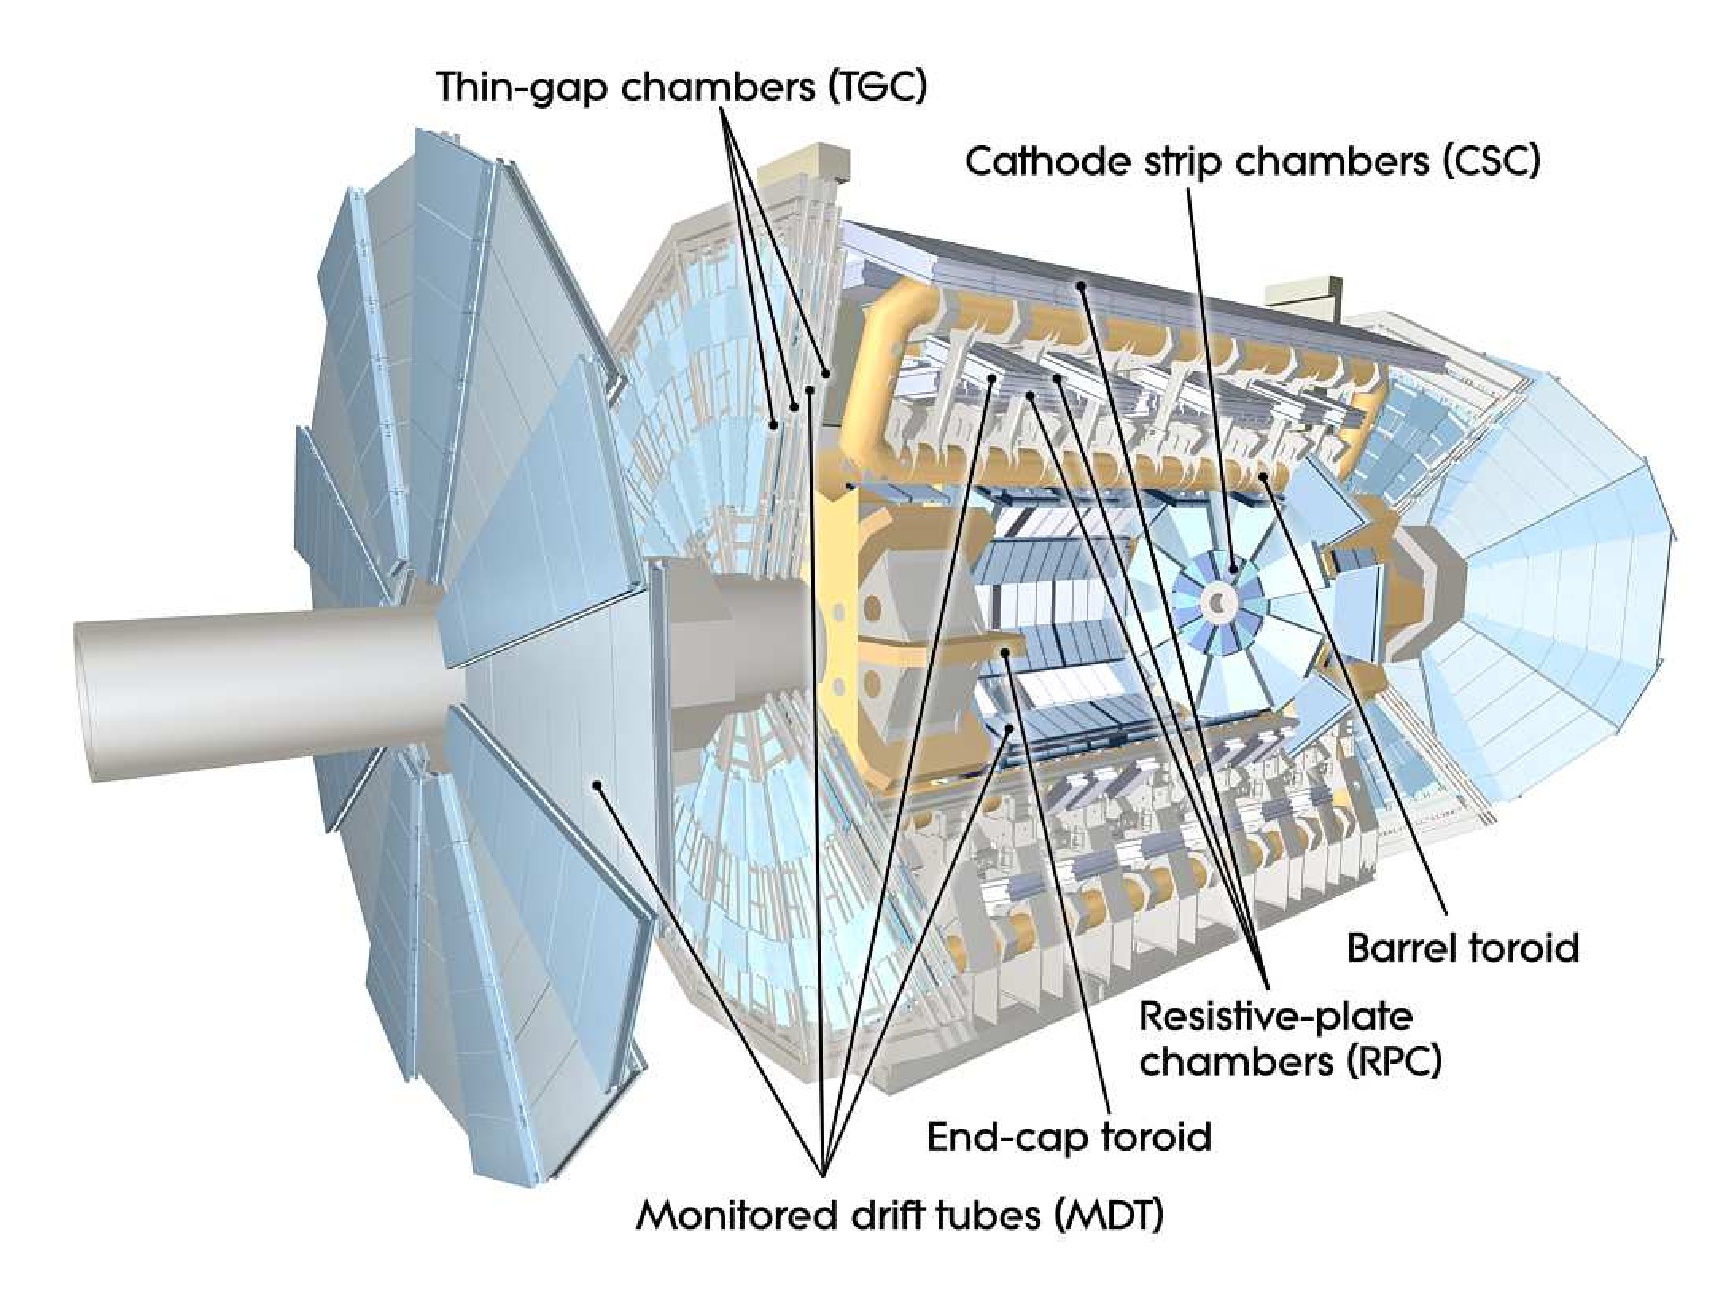
\includegraphics[width=0.7\textwidth]{figure/muonSpec.png}

    \end{center}
    \caption{Cut-away view of the ATLAS muon spectrometer system. Ref.~\cite{ATLASDetector}.}



   \label{fig:atlasMu}
\end{figure}
The muon spectrometer is instrumented with separate high-precision tracking and trigger chambers. The measure of muon momenta is performed 
by reconstructing the track curvature in an intense magnetic field produced by the large superconducting air-core toroid magnets.
The layout of the muon spectrometer is shown in Figure~\ref{fig:atlasMu}.

Precision measurement of the track coordinates in the principal bending direction of the 
magnetic field is provided by Monitored Drift Tubes (MDT’s) up to $|\eta| < 2.7$. Given the demanding rate and background conditions
at large pseudorapidities, $2 < |\eta| < 2.7$, the innermost MDT layer is replaced by  Cathode Strip Chambers (CSC’s), which are multiwire
proportional chambers with cathodes segmented into strips. Precise muon momentum measurement is achieved for muons with momenta up to 1~TeV.
The best momentum resolution, 3-4\%, is achieved for muons with transverse momenta $\sim 100$~GeV, while resolution of $\sim 10\%$ are reached for muons
with momenta up to 1~TeV. 

The trigger system covers the pseudorapidity range $|\eta| < 2.4$. Resistive Plate Chambers
(RPC’s) are used in the barrel and Thin Gap Chambers (TGC’s) in the end-cap regions for the trigger information. 


\subsection{The Trigger System}
The trigger system has three distinct levels: L1, L2, and the event filter (EF). Each trigger level
refines the decisions made at the previous level and, where necessary, applies additional selection
criteria.

The L1 trigger searches for high transverse-momentum muons, electrons, photons, jets, and $\tau$ 
leptons decaying into hadrons, as well as large missing and total transverse energy.
Its selection is based on information from the set of detectors described previously.
The L1 trigger defines in the interesting events one or more Regions-of-Interest (RoI), given by $\eta-\phi$ coordinates
of interesting feature of the event.

The L2 selection is seeded by the RoI information provided by the L1 trigger, it uses the full granularity and precision of 
all the available detector data within the RoI’s. The L2 triggers are designed to reduce the
trigger rate to approximately $3.5\,\text{kHz}$.

The final stage of the event selection is carried out by the event filter, which reduces
the event rate to roughly 200 Hz. Its selections are implemented using offline analysis and reconstruction procedures.


\subsection{Luminosity Measuremet}
A precise measurement of the recordered integrated luminosity is extremely important for all the physics measuremens of the ATLAS physics program.

Several technique are employed in ATLAS for the measure of the luminosity, the most relevant detectors that  monitor the 
luminosity are the Inner Detector, the BMC and the LUCID detectors. For a detalied description of the ATLAS luminosity measurements
and their performance see Ref.~\cite{luminosity}.
The Inner Detector measure the luminosity by the averange reconstructed proton-proton interaction per buch crossing.
The LUCID detector surrounds the beampipe on both sides of the interaction point at a distance of 17 m, providing whit its Cherenkov
detectors the measures of the particle flux from the interaction point in a very forward region. The BCM counts the number of collision per 
bunch crossing providing an independent luminosity estimate.











